\section{Introduction}

% TODO show a mesh structure. (dolphin from Wikipedia maybe)

% Overview
  % Environmental mapping, what is the motivation?
  % Maps
  % RGBD sensors
% Goal

\begin{frame}{Motivation} % ____________________________________________________

  SLAM problem

  \medskip

  Environmental mapping provides situational awareness for:
  \begin{itemize}
    \item Autonomous agent
    \item Teleoperation
  \end{itemize}

  \begin{center}
  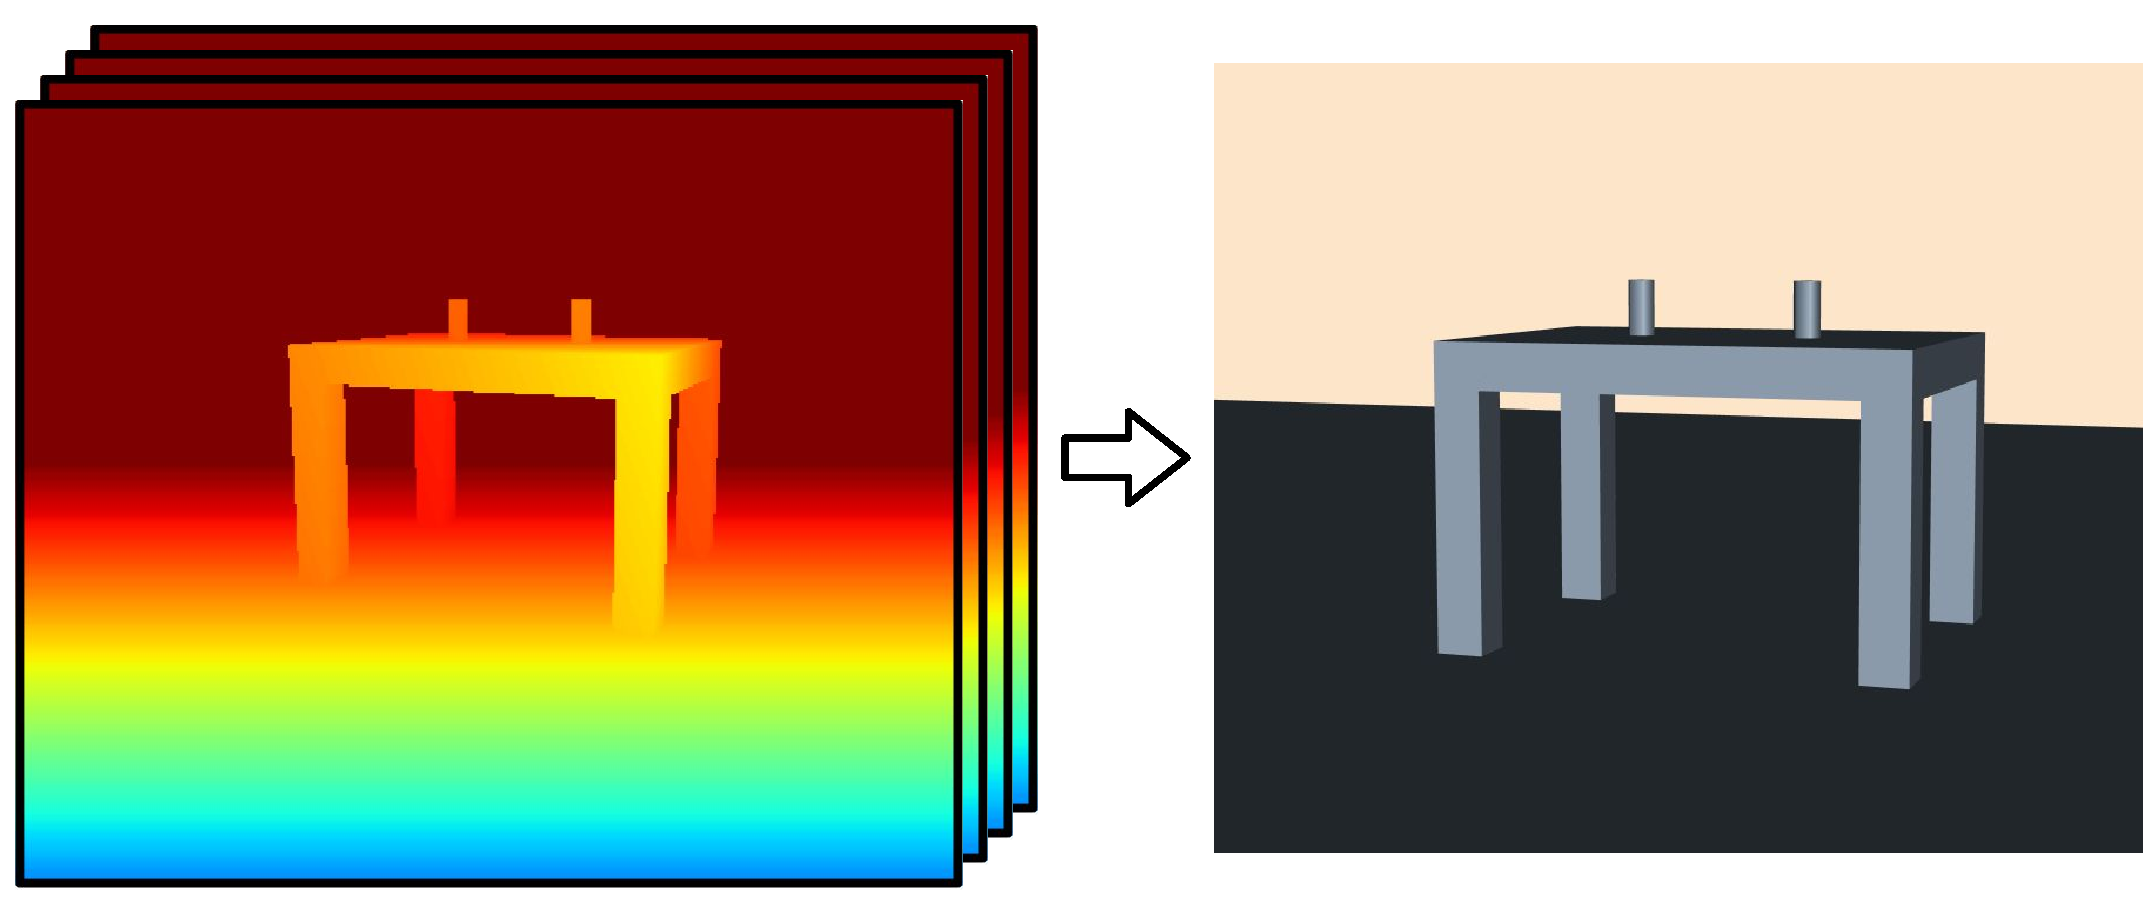
\includegraphics[width=\textwidth]{../figures/intro_goal.pdf}
  \end{center}
\end{frame}

\note[itemize]{
\item This work is in the field of Environmental Planning
\item In general Environmental Planning provides situational awareness
\item Examples Autonomous - Path planning, obstacle avoidance, object manipulation
\item Examples Teleoperation - Search and Rescue, Hazardous Environments
}


\begin{frame}{Pipeline} % ______________________________________________
  \hspace*{-12.5mm}
  \includegraphics[width=1.2\textwidth]<1>
    {../figures/intro_general_pipeline_blackbox.pdf}
  \includegraphics[width=1.2\textwidth]<2>
    {../figures/intro_general_pipeline_mabdi.pdf}

  \note<1>{\begin{itemize}
    \item Traditional Methods
  \end{itemize}}

  \note<2>{\begin{itemize}
    \item MABDI
  \end{itemize}}
\end{frame}
